\documentclass{article}

\usepackage{graphicx}
\usepackage{tikz}
\usepackage{tikzsymbols}
\usetikzlibrary{calc,patterns,shapes.geometric}
\pagestyle{empty}
\usepackage[margin=0pt]{geometry}
\geometry{papersize={14in,12in}}

\def\centerarc[#1](#2)(#3:#4:#5){\draw[#1] ($(#2)+({#5*cos(#3)},{#5*sin(#3)})$) arc (#3:#4:#5);}

\begin{document}
	\begin{figure}
		\centering
		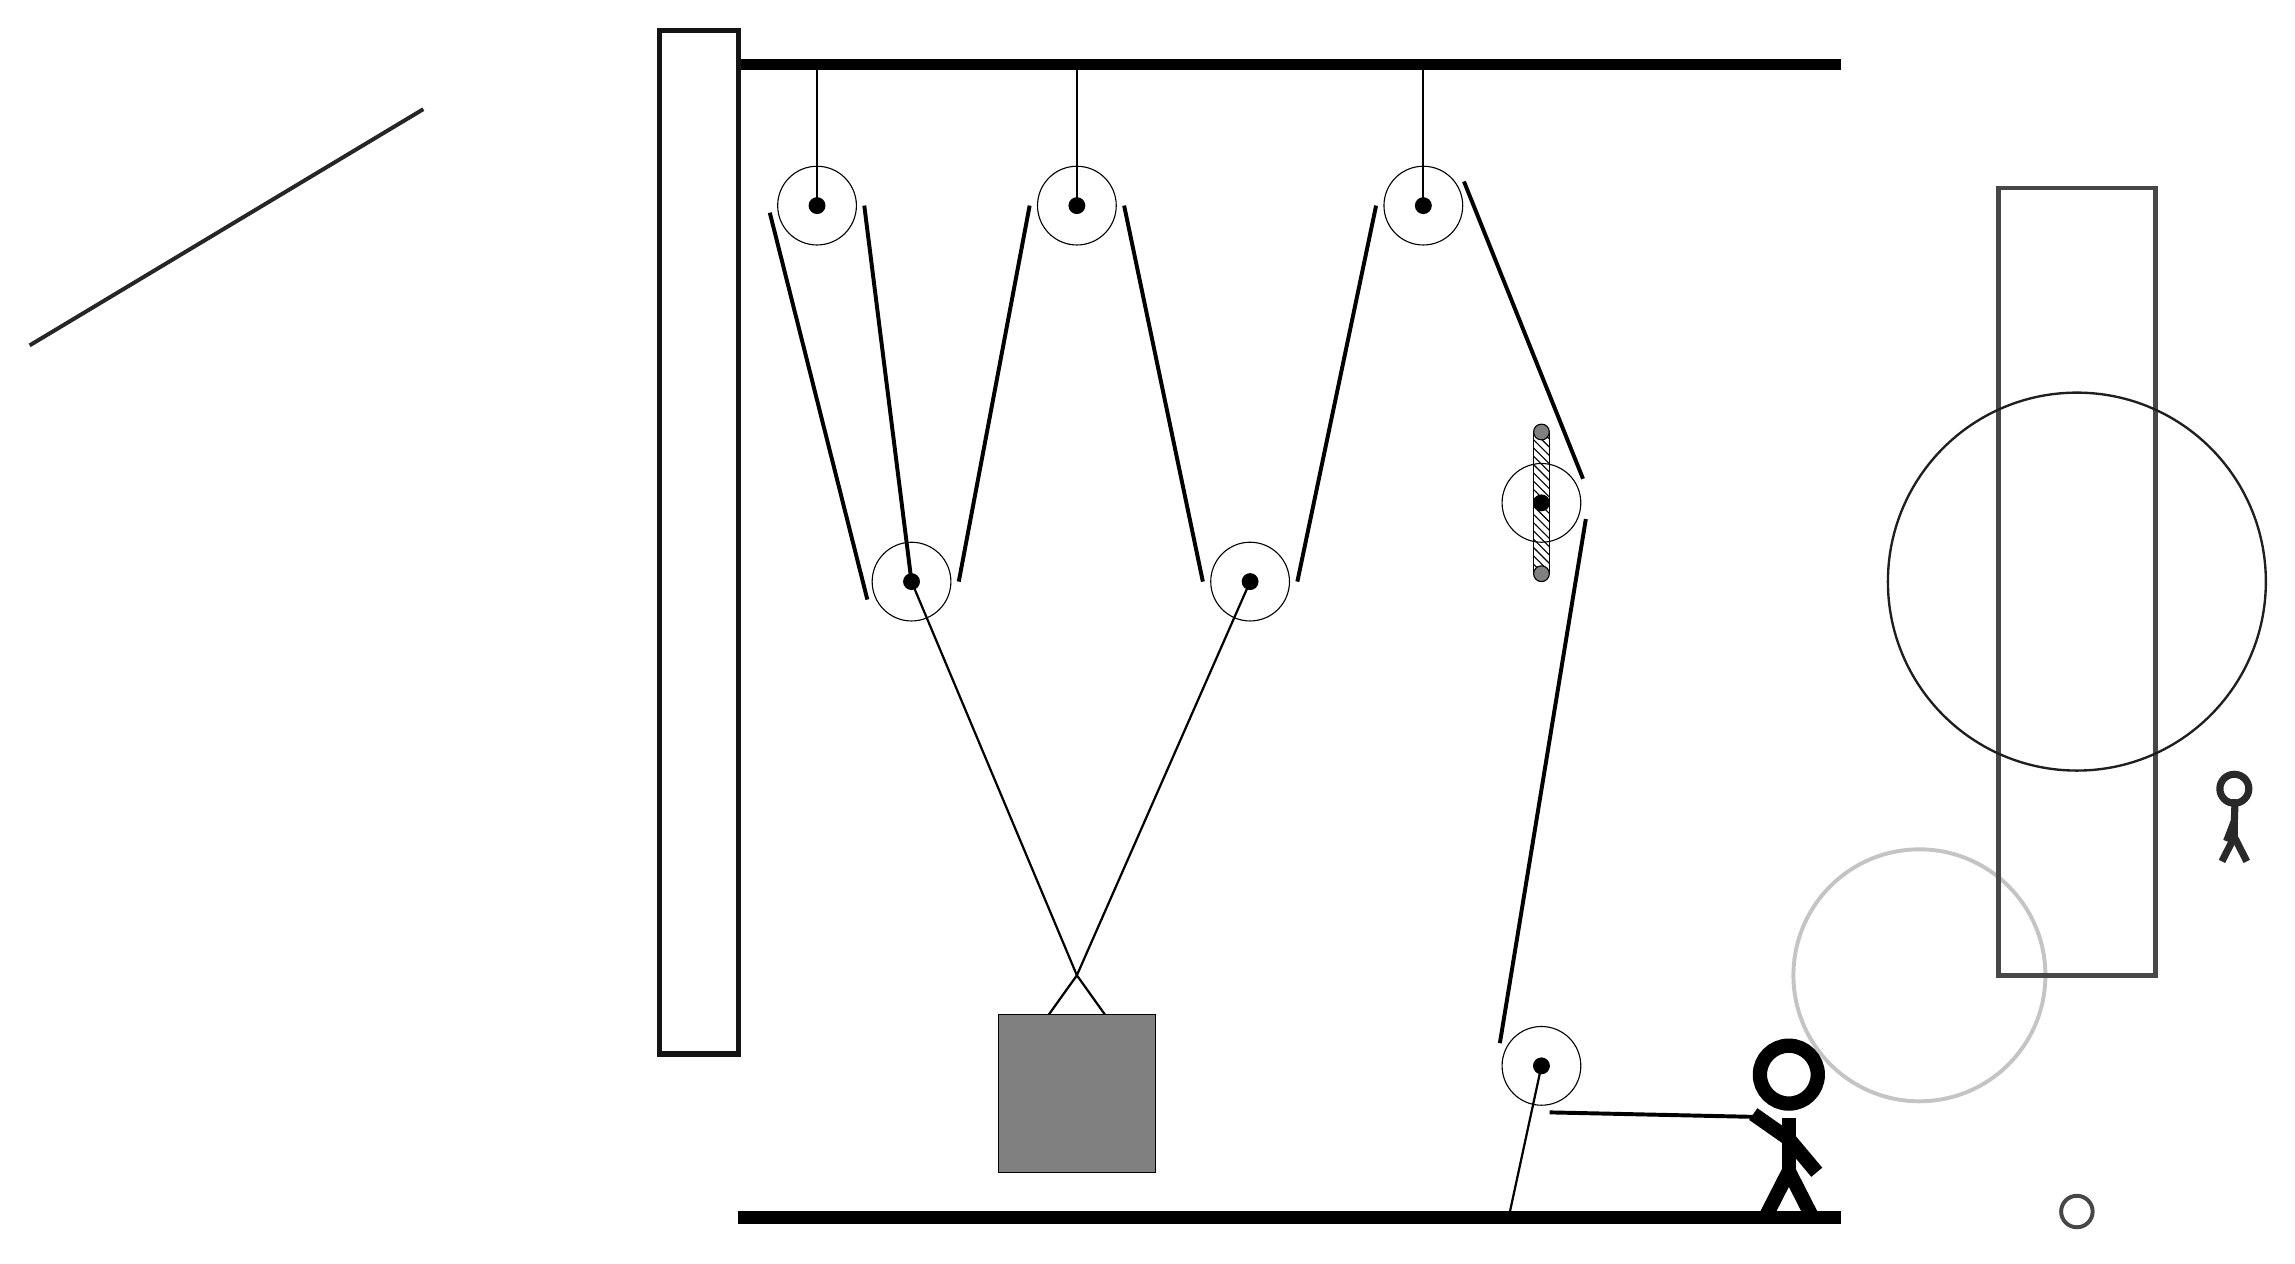
\begin{tikzpicture}
			%%%%% START %%%%%
			
			\draw[fill=black] (-2, 11.5) rectangle (12, 11.625);
			
			\draw (-1, 9.775) circle (0.5);
			\draw[fill=black] (-1, 9.775) circle (0.1);
			\draw[thick] (-1, 9.775) -- (-1, 11.5);
			
			\draw (2.3, 9.775) circle (0.5);
			\draw[fill=black] (2.3, 9.775) circle (0.1);
			\draw[thick] (2.3, 9.775) -- (2.3, 11.5);
			
			\draw (6.7, 9.775) circle (0.5);
			\draw[fill=black] (6.7, 9.775) circle (0.1);
			\draw[thick] (6.7, 9.775) -- (6.7, 11.5);
			
			\draw (0.2, 5) circle (0.5);
			\draw[fill=black] (0.2, 5) circle (0.1);
			
			\draw (4.5, 5) circle (0.5);
			\draw[fill=black] (4.5, 5) circle (0.1);
			
			\draw (8.2, 6.0) circle (0.5);
			\draw[fill=black] (8.2, 6.0) circle (0.1);
			\draw[pattern=north west lines, pattern color=black] (8.1, 6.9) rectangle (8.3, 5.1);
			\draw[fill=black!50] (8.2, 6.9) circle (0.1);
			\draw[fill=black!50] (8.2, 5.1) circle (0.1);
			
			\draw [line width=0.5mm, color=black!23](13, 0) circle (1.6);
			
			\draw[line width=0.7mm, color=black!92] (-2, 12) rectangle (-3, -1);
			\draw [line width=0.5mm, color=black!72](15, -3) circle (0.2);
			\draw[line width=0.5mm, color=black!42](14, 0) -- (14, 7);
			
			\node[line width=0.6mm, color=black!84] at (17, 2) {\Strichmaxerl[5][69][88]};
			\draw[line width=0.6mm, color=black!72] (14, 10) rectangle (16, 0);
			\draw [line width=0.3mm, color=black!88](15, 5) circle (2.4);
			\draw[line width=0.5mm, color=black!85](-6, 11) -- (-11, 8);
			
			\draw (8.2, -1.15) circle (0.5);
			\draw[fill=black] (8.2, -1.15) circle (0.1);
			\draw[thick] (8.2, -1.15) -- (7.8, -3);
			
			\draw[thick] (0.2, 5) -- (2.3, 0)  -- (4.5, 5);
			\draw[thick]  (1.8, -0.7) -- (2.3, 0) -- (2.8, -0.7);
			\draw[fill=black!50] (1.3, -0.5) rectangle (3.3, -2.5);
			\draw[line width=0.5mm] (0.2, 5) -- (-0.4, 9.775);
			\centerarc[line width=0.5mm](-1, 9.775)(0:200:0.6);
			\draw[line width=0.5mm] (-1.6, 9.685) -- (-0.361, 4.772);
			\centerarc[line width=0.5mm](0.2, 5)(200:360:0.6);
			\draw[line width=0.5mm](0.8, 5) -- (1.7, 9.775);
			\centerarc[line width=0.5mm](2.3, 9.775)(0:180:0.6);
			\draw[line width=0.5mm] (2.9, 9.775) -- (3.9, 5);
			\centerarc[line width=0.5mm](4.5, 5)(180:360:0.6);
			\draw[line width=0.5mm] (5.1, 5) -- (6.1, 9.775);
			\centerarc[line width=0.5mm](6.7, 9.775)(30:180:0.6);
			\draw[line width=0.5mm](7.216, 10.081) -- (8.728, 6.306);
			\centerarc[line width=0.5mm](8.2, 6.0)(160:211:-0.6);
			\draw[line width=0.5mm](8.7638, 5.7948) -- (7.672, -0.862);
			\centerarc[line width=0.5mm](8.2, -1.15)(150:280:0.6);
			\draw[line width=0.5mm](8.3042, -1.7409) -- (11, -1.8);
			
			\node at (11.3, -2) {\Strichmaxerl[10][-35][-50]};
			
			\draw[fill=black] (-2, -3) rectangle (12, -3.15);
			
			%%%%% END %%%%%
		\end{tikzpicture}
	\end{figure}	
\end{document}